\documentclass[../main]{subfiles}
\begin{document}

\section{Final product}
\label{s:app}

The final product for the users is a mobile application for Android devices that allows them to save their points of interest, having simple social interactions 
through the friendship requests, see and share live events with their friends and receive advices for places to visit through location-, social- and activity-aware recommendations.
The main screens of the application are the \textbf{map} and the \textbf{main menu} showed in the following pictures.
\begin{figure}[H]
    \centering
    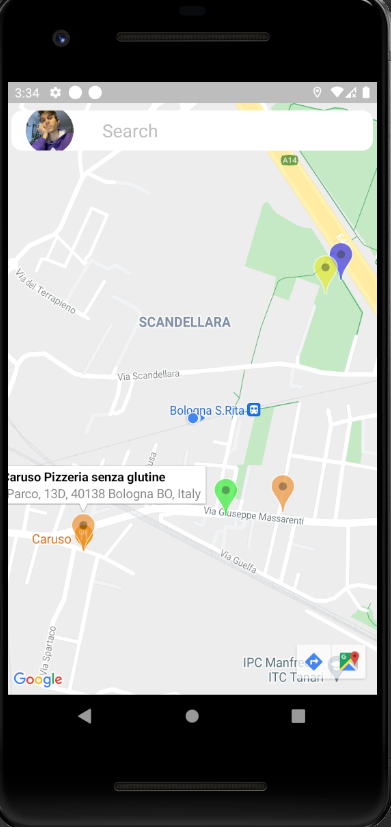
\includegraphics[width=0.4\textwidth]{images/app/app_overview}
    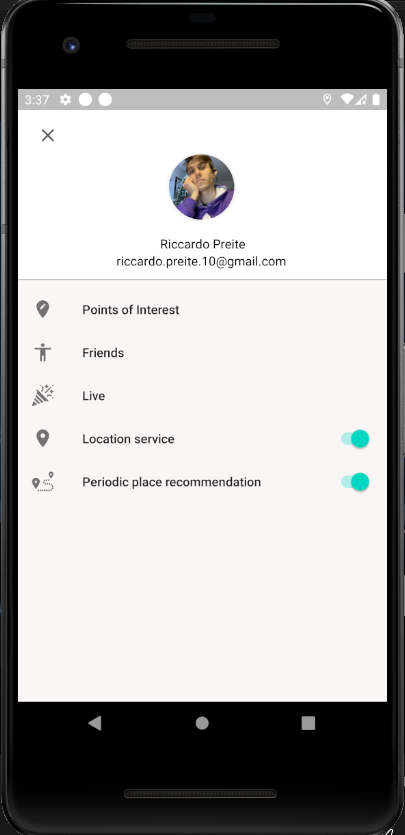
\includegraphics[width=0.41\textwidth]{images/app/main_menu}
    \caption{On the left, the map with some \textit{pois}. On the right, the main menu.}
\end{figure}


\subfile{04_app/04_1_poi}
\subfile{04_app/04_2_friend}
\subfile{04_app/04_3_live}
\subfile{04_app/04_4_recommendation}

\end{document}